
La detección de muones en este proyecto es realizada mediante un detector de partículas inspirado en los detectores sTGC del experimento ATLAS, como se mencionó en la Sección \ref{par:smallwheel}. Los detectores originales se ubican en la llamada Small Wheel de ATLAS, formando parte del Espectrómetro de Muones, el cual se encarga de determinar el momento y la trayectoria de los muones emitidos por las colisiones. Para el proyecto sTGC minería, CCTVal construyó un prototipo de detector sTGC a menor escala utilizando la misma tecnología de fabricación presente en los detectores originales. En esta sección se describe la estructura de un sTGC original y la del prototipo en cuestión, incluyendo información sobre el funcionamiento y operación del prototipo de detector sTGC fabricado en CCTVal.

\begin{figure}[h]
	\centering
	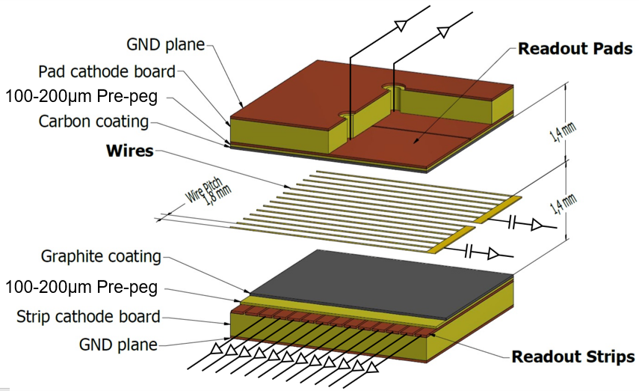
\includegraphics[scale=0.7]{tgc-structure.png}
	\caption{Estructura interna de un detector TGC\cite{Chapman2014ATLASUpgrade}.}
	\label{img:stgc-structure}
\end{figure}

\subsection{Estructura general} 
	Un sTGC está compuesto por dos planos de grafito (cátodos), con múltiples cables en medio (ánodos)\cite{Formenti2018CERNReport}, tal como se observa en la Figura \ref{img:stgc-structure}. Recubriendo el exterior de ambos cátodos se ubican capas aislantes que separan los cátodos de las zonas conductoras, llamadas ``\textit{pads}'' en la cara superior y ``\textit{strips}'' en la cara inferior del detector, diferenciándose en la forma y área que abarca cada uno. Los \textit{strips} corresponden a delgados rectángulos de cobre, mientras que los \textit{pads} son mantos de cobre más anchos, equivalentes al área de varios \textit{strips}. Los cables al interior del detector se encuentran orientados perpendicularmente respecto a los \textit{strips} y en paralelo a los \textit{pads}.
	
	Al interior del detector, entre los planos de grafito, se infiltra un gas compuesto por dióxido de carbono y n-pentano\cite{Formenti2018CERNReport}. Mediante la aplicación de alto voltaje se genera un campo eléctrico entre ánodos y cátodos. Se utilizan 3000 V$_{DC}$ entre cátodos y ánodos para generar el campo eléctrico, limitando la corriente a 50uA. El gas en el interior puede ser dióxido de carbono puro, pero esto genera mayor probabilidad de generar descargas no asociadas a muones. La Figura \ref{img:stgc-field} representa un corte transversal de un detector y sus líneas de campo eléctrico desde ánodo (cables) hasta cátodos (lámina de grafito superior e inferior). 
	
	El paso de muones a través del detector genera la ionización del gas y la liberación de electrones, los cuales son captados por los cables del detector gracias al campo eléctrico. El flujo de electrones en el gas ionizado genera pulsos de corriente en los cables, produciendo diferencia de potencial en los cátodos. Esta diferencia de potencial interactúa con los \textit{pads} y \textit{strips} en el exterior del detector, generando pulsos de voltaje en estas zonas conductoras, pero con polaridad inversa respecto a la corriente presente en los cables. En la Figura \ref{fig:sistema-completo}, el pulso de voltaje correspondiente a la señal de salida de un canal de detección está representado por el pulso verde dibujado en la zona central de la imagen.
	
	La amplitud de los pulsos generados en el detector será mayor en torno al vértice de interacción y menor en zonas lejos de él. Esto permite relacionar la posición y energía de la partícula con las amplitudes de los pulsos en cada \textit{strip} o cable medido.
	
	\begin{figure}[h]
		\centering
		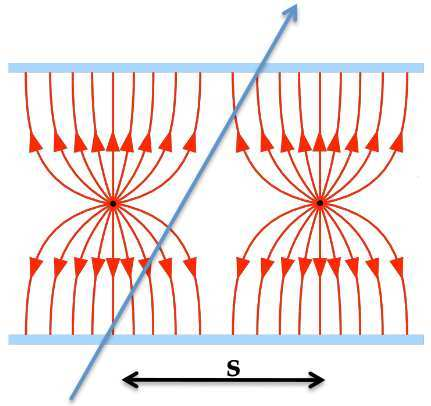
\includegraphics[scale=0.3]{stgc-transversal.png}
		\caption{Lineas de campo eléctrico observadas en un corte transversal de los cables y cátodos del detector. Los cátodos se ilustran en celeste, los cables se representan como puntos negros, y las lineas de campo corresponden a las flechas de color rojo\cite{DeSmet2011StudyLab}.}
		\label{img:stgc-field}
	\end{figure}

\subsection{Detector sTGC utilizado}
	En ATLAS, los vértices de interacción se determinan leyendo las señales provenientes de \textit{strips} y cables al mismo tiempo. Debido a que los \textit{strips} son perpendiculares a los cables, su lectura forma un cuadrante imaginario de dos ejes coordenados (\textit){strips} vs. cables), similar al presentado en la Figura \ref{img:cuadrantes-ministgc}. Por ejemplo, si un muon interactúa con un cable y un \textit{strip} al mismo tiempo, significa que el vértice de interacción se ubica en las cercanías de la intersección \textit{strip}/cable. Sin embargo, para el trabajo considerado en esta memoria de titulación se leerán solo las señales provenientes de \textit{strips}, por los que se estará midiendo un solo eje de posición y será necesario agregar un segundo eje coordenado para poder determinar los vértices de interacción. La ventaja de leer señales desde \textit{strips} es que las señales medibles en ellos son de fácil acceso, debido a que los \textit{strips} son superficies conductoras expuestas al exterior y permiten incorporar conectores sobre ellos sin mayor dificultad.
	
	Para agregar un eje coordenado adicional al detector, se reemplazan los \textit{pads} de la cara superior por \textit{strips} perpendiculares a los del plano contrario. Así se logra tener información bidimensional del paso de una partícula leyendo solo las señales provenientes de \textit{strips} perpendiculares entre sí. La Figura \ref{img:stgc-mini-estructura} ilustra la composición del detector capa por capa y detalla la orientación de cables y \textit{strips}.
	
	\begin{figure}[h]
		\centering
		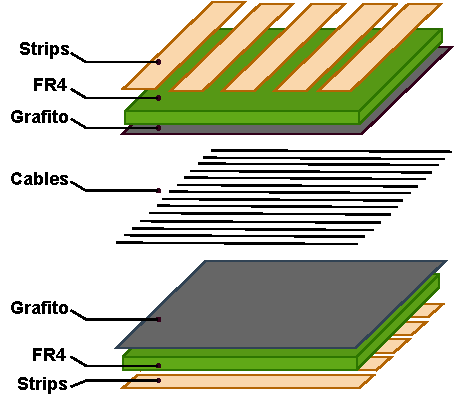
\includegraphics[scale=1]{stgc-mini-estructura}
		\caption{Estructura interna de un detector sTGC adaptado para este proyecto de titulación. El gas es contenido entre ambas capas de grafito (cátodos). Los cables internos corresponden a los ánodos.}
		\label{img:stgc-mini-estructura}
	\end{figure}

	En particular, en cada cara del detector utilizado se cuenta con 8 \textit{strips} de 15cm de largo y 1cm de ancho cada uno, sin contar los \textit{strips} en los bordes del detector debido a que el área abarcada por estos es diferente a la forma de un \textit{strip} estándar, entorpeciendo la medición y posterior reconstrucción de datos. %\sgcnote{hay strips inutiles?}\jgnote{efectivamente}.
Una fotografía de este detector se incluye en la Figura \ref{img:foto-mini-stgc}. En la parte superior de la fotografía, en recuadros verdes, se observan tubos para el flujo de gas. Por abajo, en amarillo, se indican 8 cables coaxiales conectados a los \textit{strips} de la cara superior del detector. A la izquierda están situados los otros 8 cables correspondientes a los \textit{strips} de la cara inferior, también etiquetados en amarillo. En el costado derecho, en el recuadro azul, existe una red resistiva para la lectura de cables internos del detector, los cuales no serán utilizados en este proyecto. % \sgcnote{marcar claramente estas componentes en la figura.}.
	
	\begin{figure}[h]
		\centering
		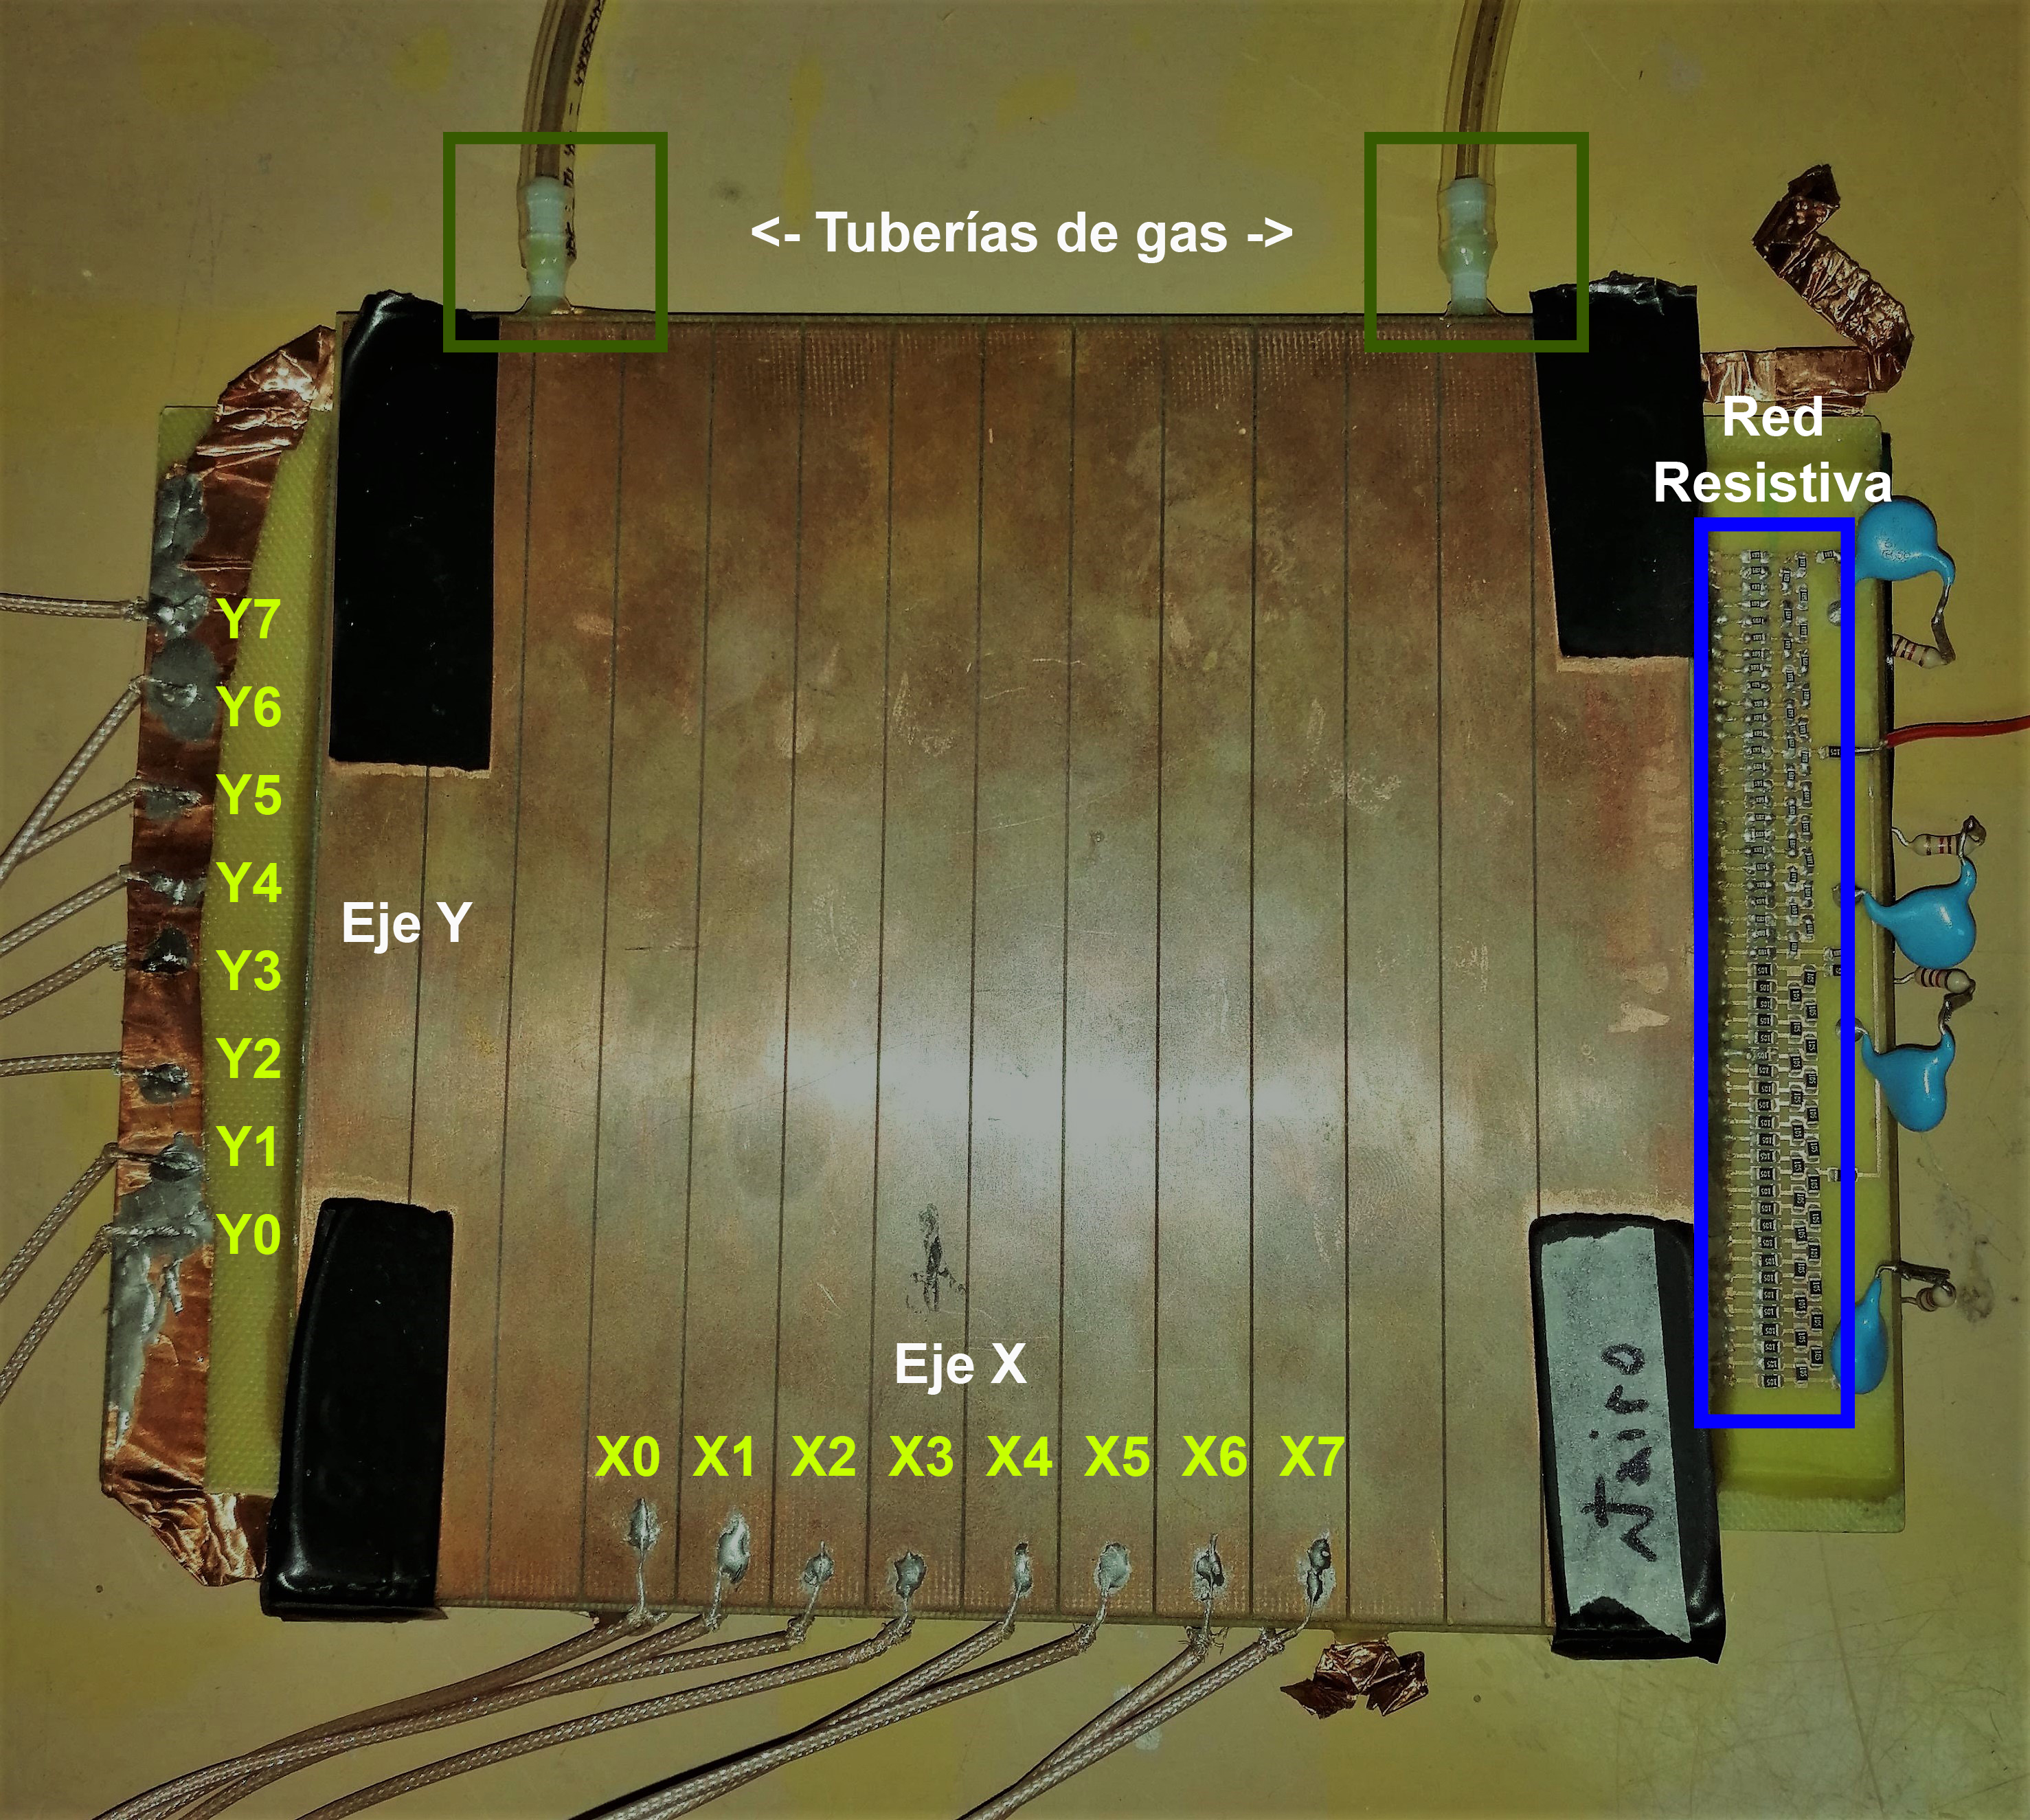
\includegraphics[scale=0.08]{mini-stgc2.jpg}
		\caption{Vista superior del detector prototipo.}
		\label{img:foto-mini-stgc}
	\end{figure}	
	
	Dado que los \textit{strips} de la cara superior del detector son perpendiculares a los de la cara inferior, es posible interpretar el detector como un cuadrante de ejes coordenados según se ilustra en la Figura \ref{img:cuadrantes-ministgc}. En esta figura, cada cuadro representa un área de detección de 1cm$^2$, la cual corresponde a la precisión para la determinación de los vértices de interacción. Como el detector posee 8 \textit{strips} por cara, se tiene un total de 16 canales de detección, los que en su conjunto forman 64 zonas de detección de 1cm$^2$. Los \textit{strips} de la cara superior se nombrarán como el eje X, mientras que los \textit{strips} correspondientes a la cara inferior del detector serán asociados al eje Y, siendo el cuadro (0,0) aquel que se ubica en la zona de detección inferior izquierda.
	
	\begin{figure}[h]
		\centering
		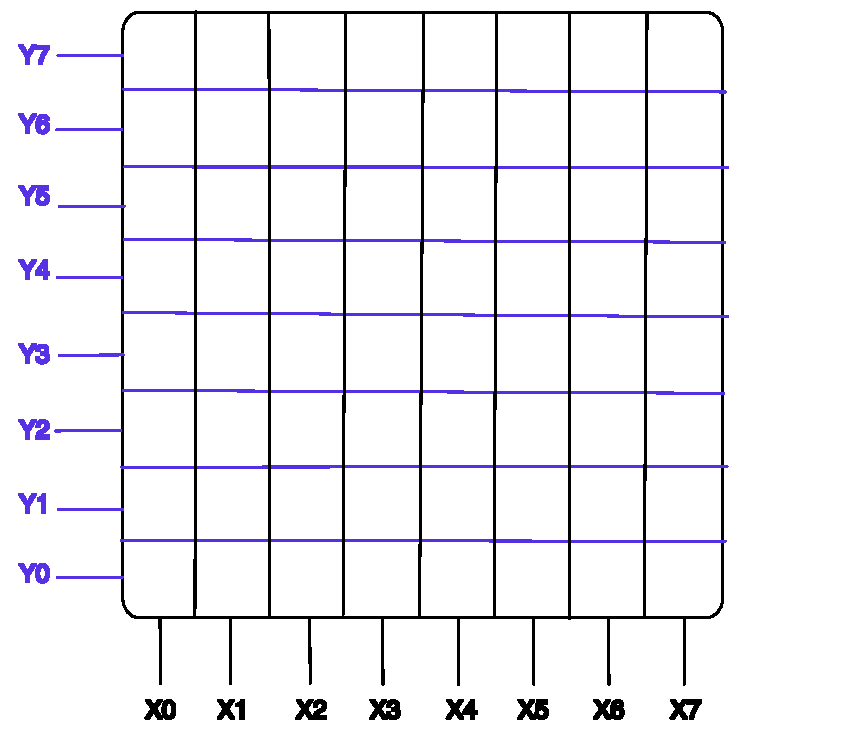
\includegraphics[scale=0.55]{cuadrantes-ministgc.pdf}
		\caption{Vista superior del detector, en donde se indican las etiquetas asociadas a cada canal en función del eje al que pertenece. Cada cuadro representa un área de detección de 1cm$^2$.}
		\label{img:cuadrantes-ministgc}
	\end{figure}

\subsection{Procedimiento de Operación y Pruebas}
	Antes de poner en marcha mediciones o experimentos con un nuevo detector, se deben realizar ajustes, caracterizaciones y pruebas que permitan corroborar el correcto funcionamiento del dispositivo. Para esto, se recomienda llevar a cabo una secuencia de experimentos con el fin de comprobar el funcionamiento de cada canal y medir el ruido base, la frecuencia de detección y las amplitudes medias esperadas.

	\subsubsection{Dispositivos para lectura de señales}
		Para observar los pulsos captados por el detector es necesario contar con un sistema de lectura adecuado. Este dispositivo deberá poseer una  baja impedancia, menor a 100$\Omega$ para evitar atenuaciones y reflexiones, así como también deberá contar con una etapa de amplificación tal que permita medir sin problemas las señales captadas con un osciloscopio, digitalizador o un sistema para adquisición de datos. Las señales emitidas por el detector rondan el orden de los milivolts, lo cual significa que el sistema de lectura debe poseer una ganancia tal que la magnitud de la señal de salida esté dentro de la resolución de voltaje del aparato de medición.
		
		Un ejemplo de sistema de lectura es la interfaz ASD mencionada en la Sección \ref{sec:atlas}, la cual será utilizada en este proyecto de titulación. Esta interfaz está diseñada para la correcta lectura de \textit{strips} y cables provenientes de detectores TGC, contando con una amplificación inicial de 0.8V/pC de carga y con una segunda etapa capaz de amplificar 7 veces la señal entrante. Además, la primera etapa de amplificación de la interfaz ASD se encarga de darle forma al pulso captado, con el fin extender la señal en el tiempo y facilitar su muestreo.
		
		%La interfaz ASD cuenta con salidas digitales de tipo LVDS. Estas señales representan el tiempo que la señal permanece por sobre un umbral arbitrario configurado, el cual será proporcional a la amplitud y por tanto a la carga del pulso medido. Cuenta también con una única señal análoga conectada al canal 16 (\textit{Hit} 15), proveniente de la pre-amplificación. Esta es una señal de monitoreo ideal para realizar pruebas de funcionamiento.
		

	\subsubsection{Estimación de ruido base}
		Una vez escogidos los métodos de lectura y las herramientas de muestreo a utilizar, es necesario medir el ruido base del detector. Este ruido corresponde a distorsiones propias del dispositivo, como fugas de corriente, conducción indeseada y ruido electromagnético. Conocer el ruido base permite filtrar el ruido para el análisis de eventos de interés.
		
		Para realizar la medición de ruido base en este detector prototipo se debe hacer circular el dióxido de carbono (o mezcla de dióxido de carbono y N-Pentano). Antes de proceder a realizar mediciones, es necesario esperar a que el detector haya sido llenado totalmente de gas. Dada su área interior cercana a los 225cm$^2$, el detector se encontrará completamente infiltrado con gas tras 20 minutos de operación. %\sgcnote{Especificar que estos son pasos y procedimientos para el detector en particular.  Como estan, suenan muy absolutos, como que siempre se deb hacer asi y no hay otra forma.}
		
		Cuando el detector se encuentra totalmente lleno de gas, se procede a medir el ruido base en cada uno de sus canales, sin conectar el detector a su fuente de alto voltaje. Estas mediciones permiten generar histogramas de ruido, los cuales han de tener una distribución gaussiana en condiciones normales de operación. \gcnote{Puedes mostrar resultados de esto?}\jgnote{lamentablemente no tengo datos para mostrar, es parte de las pruebas de caracterización del detector que se deben realizar de manera presencial de un laboratorio, pero encontre una referencia del proyecto ATLAS donde se observa ruido base en un histograma junto a otros datos sin indicar su distribución de manera explicita. Servira?}
		
		La amplitud del ruido base definirá una zona que deberá ser considerada en los análisis de eventos. Pulsos dentro de este rango de amplitudes no serán correctamente captados. Por otro lado, se espera que el ruido sea menor que la amplitud media de los eventos generados por cruce de muones en el detector.
		
		Conocer tanto la amplitud del ruido base como la de los pulsos originados por muones, permite escoger señales de disparo en la tarjeta ASD, o filtros digitales en las etapas de análisis. 
		
	\subsubsection{Observación de falsas detecciones}
		Para una fiel interpretación de la información captada por un detector, es importante conocer la distribución y frecuencia de detecciones que no correspondan a cruce de muones. La medición de estos parámetros requiere la generación del campo eléctrico dentro del detector conectando su respectiva fuente de alto voltaje.
		
		Una vez generado el campo eléctrico, es posible captar falsas detecciones o disparos aleatorios producto de la conductividad de los materiales o fugas de corriente. Estos eventos suelen tener una distribución normal y ser de amplitudes mayores a la de interés (muones). Conocer esta información permite ignorar señales sobre un umbral tal que se correspondan con amplitudes de eventos no deseados.
	
	\subsubsection{Detección de partículas}
		Para comprobar el correcto funcionamiento del detector, es de gran utilidad utilizar fuentes radioactivas para generar pulsos de prueba. Aunque una fuente radioactiva de rayos Gamma genera pulsos de mayor amplitud que eventos producidos por muones, esta permite comprobar la correcta operación de cada canal y la distribución de carga del evento en cada canal adyacente.
	
		Para el caso de detección de muones, es importante contar con un sistema de disparo para ignorar detecciones provenientes de otras partículas cargadas capaces de ionizar el gas al interior del detector. Para el caso de sTGC, se cuenta con el sistema de detectores centelladores mencionados con anterioridad e ilustrados en la Figura \ref{fig:sistema-completo}. Se recomienda posicionar uno de estos detectores sobre el detector sTGC, cubriendo un área igual a la que abarque el sTGC. De ser factible, se recomienda incluir un segundo detector centellador por debajo, para generar una señal de disparo conjunta con el centellador superior. Esto permite descartar incidencias casi horizontales de muones, pasando por un centellador pero no por el detector sTGC.
		